\chapter[Радиостанции]{Радиостанции}
\label{ch:radio-station}

Радиостанции --- комплекс устройств и сооружений, служащих для подготовки программ радиовещания. 
Эта глава посвящена исследованию программ радиовещания, 
анализируется объект Викиданных \wdqName {<<вещательная радиостанция>>}{14350} и его свойства. 
Получен список всех радиостанций, описанных в Викиданных. 
С помощью запросов получено количество радиостанций у различных стран, 
определены подклассы радиостанций. 
Найдены радиостанции, вещательные каналы и~СМИ в~СССР и~России, 
выделены группы тематической направленности, 
представлены аккаунты в~социальных сетях.

\section{Число радиостанций по странам}

Получим список всех радиостанций с~указанием страны, к которой они относятся, 
посредством свойства \wdProperty{495}{<<страна происхождения>>}. 
Запрос~\ref{lst:all_radio_stations} вернул около 100 станций, 
что является недостаточным числом для радиовещательных программ всего мира, представленных в Викиданных.

\begin{lstlisting}[ 
    language=SPARQL,
    caption={\href{https://w.wiki/5unA}{Cписок всех радиостанций со свойством <<страна происхождения>>}\protect\footnotemark},
    label=lst:all_radio_stations,
    texcl,
    numbers=none
    ]
# List of radio stations and country
SELECT ?radio ?radioLabel ?countryLabel WHERE
{
  ?radio wdt:P31 wd:Q14350; # instance of radio station
         wdt:P495 ?country. # country of origin
  SERVICE wikibase:label { bd:serviceParam wikibase:language "ru,en" }
}
\end{lstlisting}%
\footnotetext{Получено: 118 результатов на 2024 год. 
              Ссылка на SPARQL-запрос: \href{https://w.wiki/9qag}{https://w.wiki/9qag}.}


Посмотрим количество радиостанций у~разных стран в~запросе~\ref{lst:NStationsCountryP495}.
Суммируем число станций в~переменную \lstinline|?sumRadio| 
с~помощью команды \lstinline|COUNT()| в~строке~2. 
Сгруппируем станции по~странам с~помощью команды \lstinline|GROUP BY| в~строке~7.


        \lstset{escapeinside={(*@}{@*)}}
        \sethlcolor{pink}

\begin{lstlisting}[ 
    language=SPARQL,
    caption={\href{https://w.wiki/9qau}
                  {Количество радиостанций со свойством <<страна происхождения>>
                   по странам}\protect\footnotemark},
    label=lst:NStationsCountryP495,
    xleftmargin=18pt,
    numbers=left,
    ]
# Number of radio stations for each country 
SELECT ((*@\hl{COUNT}@*)(?radio) as (*@\hl{?sumRadio}@*)) ?countryLabel WHERE {
  ?radio wdt:P31 wd:Q14350; # is radio station
         wdt:P495 ?country. # has country of origin
  SERVICE wikibase:label { bd:serviceParam wikibase:language "ru,en" }
}
(*@\hl{GROUP BY}@*) ?countryLabel
ORDER BY DESC (?sumRadio)
\end{lstlisting}%
\footnotetext{Получено: 31 страна с радиостанциями на 2024 год. 
              Ссылка на SPARQL-запрос: \href{https://w.wiki/9qau}{https://w.wiki/9qau}.}

Всего в мире около двухсот стран (смотри главу <<\nameref{ch:country}>> 
на~с.~\pageref{ch:RussiaNotCountryPPS}), 
но запрос~\ref{lst:NStationsCountryP495} нашёл только 31 страну с~радиостанциями. 
По-видимому, свойство \wdProperty{495}{<<страна происхождения>>} больше подходит для~указания 
<<страны происхождения творческого произведения или другого продукта>>, 
что и~указано в~описании этого свойства. 


\begin{margintable}
\caption{Страны с наибольшим числом радиостанций на 2024 год}
\begin{tabular}{|c|c|c|}
\hline
\textnumero & Количество & Страна \\
\hline
1 & 15847 & США \\
2 & 1567 & Мексика \\
3 & 1310 & Канада \\
4 & 980 & Филиппины \\
5 & 824 & Великобритания \\
6 & 734 & Бразилия \\
7 & 584 & Германия \\
8 & 464 & Австралия \\
9 & 427 & Франция \\
10 & 371 & Индия \\
\ldots & \ldots & \ldots \\
23 & 87 & Россия \\
\ldots & \ldots & \ldots \\
32 & 55 & Нидерланды \\
\ldots & \ldots & \ldots \\
\hline
\end{tabular}
\label{tab:number_of_radio_stations}
\end{margintable}


Заменив свойство радиостанций <<страна происхождения>> 
на~свойство <<\wdProperty{17}{государство}>> 
в~строке~4 запроса~\ref{lst:NStationsCountryP17}, 
получим уже больше двухсот стран. 

\begin{lstlisting}[ 
    language=SPARQL,
    caption={\href{https://w.wiki/9qdC}
                  {Количество радиостанций со свойством <<государство>>
                   по~странам}\protect\footnotemark},
    label=lst:NStationsCountryP17,
    xleftmargin=18pt,
    numbers=left,
    ]
# Number of radio stations for each country 
SELECT (COUNT(?radio) as ?sumRadio) ?countryLabel WHERE {
  ?radio wdt:P31 wd:Q14350; # is radio station
         (*@\hl{wdt:P17}@*) ?country.  # from country
  SERVICE wikibase:label { bd:serviceParam wikibase:language "ru,en" }
}
GROUP BY ?countryLabel
ORDER BY DESC (?sumRadio)
\end{lstlisting}%
\footnotetext{Получено: 209 стран с~радиостанциями~на 2024 год. 
              Ссылка на SPARQL-запрос: \href{https://w.wiki/9qdC}{https://w.wiki/9qdC}.}

Из~этих двухсот стран в~табл.~\ref{tab:number_of_radio_stations} 
представлены страны с наибольшим числом станций. 
В Нидерландах по~запросу~\ref{lst:NStationsCountryP495} есть 69 станций 
(в~остальных 30 странах меньше десяти станций), 
а~по~запросу~\ref{lst:NStationsCountryP17}~---  всего 55 радиостанций.



\section{Подклассы радиостанций}

Найдём список подклассов радиостанций и размер подкласса 
с~помощью запроса~\ref{lst:subclasses_of_radio_stations}.

\begin{lstlisting}[ 
    language=SPARQL,
    caption={\href{https://w.wiki/9qej}
                  {Список подклассов радиостанций и размер подклассов}\protect\footnotemark},
    label=lst:subclasses_of_radio_stations,
    xleftmargin=18pt,
    numbers=left,
    ]
# List of radio subclasses and subclass sizes
SELECT ?subRadio ?subRadioLabel (COUNT(?r) AS ?count) WHERE 
{
  ?subRadio wdt:P279* wd:Q14350. # subclass of radio station
  ?r wdt:P31 ?subRadio.          # instance of this subclass
  SERVICE wikibase:label { bd:serviceParam wikibase:language "ru,en" }
}
GROUP BY ?subRadio ?subRadioLabel
ORDER BY DESC(?count)
\end{lstlisting}%

\footnotetext{Получено: 23 подкласса радиостанций на 2024 год. 
              Ссылка на SPARQL-запрос: \href{https://w.wiki/9qej}{https://w.wiki/9qej}.}

Из запроса~\ref{lst:subclasses_of_radio_stations} мы получили встречаемые подклассы радиостанций, что помогло нам понять какой подкласс наиболее актуален. 

\newpage

\section{Радиостанции, СМИ и вещательные каналы России}

Ниже представлен запрос~\ref{lst:radio_stations_broadcasting_and_mass_media_in_Russia}, который ведёт поиск радиостанций, вещательных каналов и СМИ по России, и по СССР без использования VALUES.

\begin{lstlisting}[ 
    language=SPARQL,
    caption={\href{https://w.wiki/6Lup}{Список радиостанций, вещательных каналов и СМИ в России, и СССР}\protect\footnotemark},
    label=lst:radio_stations_broadcasting_and_mass_media_in_Russia,
    xleftmargin=18pt,
    numbers=left,
    ]
# List of radio stations, broadcasting and mass media in Russia 
SELECT ?radio ?radioLabel
WHERE
{
    {?radio wdt:P31 wd:Q14350.} UNION # instance of radio station
    {?radio wdt:P31 wd:Q15265344.} UNION # instance of broadcasting
    {?radio wdt:P31 wd:Q11033.} # instance of mass media
    
    {?radio wdt:P17 wd:Q159.} UNION # in Russia
    {?radio wdt:P17 wd:Q15180.} # in USSR
    SERVICE wikibase:label { bd:serviceParam wikibase:language "ru,en". }
}\end{lstlisting}%

\footnotetext{Получено: \num{117} результатов на 2023 год. Ссылка на SPARQL-запрос: \href{https://w.wiki/9iPm}{https://w.wiki/9iPm}. }

\newpage

Расширен предыдущий запрос~\ref{lst:radio_stations_broadcasting_and_mass_media_in_Russia}. В обновленном запросе~\ref{lst:Russia_and_USSR_radio_stations_broadcasting_and_mass_media} используется функция VALUES.  Функция VALUES позволяет нам объединить свойства и уменьшить величину кода, что можно увидеть в строке №10 \lstinline|VALUES ?ruCountries {wd:Q15180 wd:Q159}|. С использованием функции UNION приходится для каждого подсвойства повторять конструкцию \lstinline|?radio wdt:P17|, что приводит к увеличению объема кода \lstinline| {?radio wdt:P17 wd:Q159.} UNION {?radio wdt:P17 wd:Q15180}|.

\begin{lstlisting}[ 
    language=SPARQL,
    caption={\href{https://w.wiki/6LU7}{Радиостанции, вещательные каналы и СМИ по России, и по СССР}\protect\footnotemark},
    label=lst:Russia_and_USSR_radio_stations_broadcasting_and_mass_media,
    xleftmargin=18pt,
    numbers=left,
    ]
# List of Russian and USSR radio stations, broadcastings and mass media
SELECT  ?radio  ?radioLabel
WHERE
{
  {?radio wdt:P31 wd:Q14350.} UNION # instance of radio station
  {?radio wdt:P31 wd:Q15265344.} UNION # instance of broadcasting
  {?radio wdt:P31 wd:Q11033.} #instance of mass media
  
  # Soviet Union and Russia
  VALUES ?ruCountries {wd:Q15180 wd:Q159}
  ?radio wdt:P17 ?ruCountries. # related to Russian countries
  
  SERVICE wikibase:label {bd:serviceParam wikibase:language "ru,en"}
}\end{lstlisting}%

\footnotetext{Получено: \num{117} результатов на 2023 год. Ссылка на SPARQL-запрос: \href{https://w.wiki/6LU7}{https://w.wiki/6LU7}. }

\newpage

\section{Тематика радиостанций России и СССР}

Данный запрос~\ref{lst:main_topics_of_radio_stations_broadcasting _and_mass_media} предназначен для поиска тематик радиостанций, СМИ и вещательных каналов.

\begin{lstlisting}[ 
    language=SPARQL,
    caption={\href{https://w.wiki/6b7P}{Поиск тематик радиостанций, СМИ и вещательных каналов}\protect\footnotemark},
    label=lst:main_topics_of_radio_stations_broadcasting _and_mass_media,
    xleftmargin=18pt,
    numbers=left,
    ]
# List of the main topics of radio stations, media and mass media
SELECT ?radio ?radioName (GROUP_CONCAT(DISTINCT ?mainSubjectLabel;separator=", ") AS ?mainSubjects) 
WHERE
{
  {?radio wdt:P31 wd:Q14350.} UNION # instance of radio station
  {?radio wdt:P31 wd:Q15265344.} UNION # instance of broadcasting
  {?radio wdt:P31 wd:Q11033.} #instance of mass media
  
  # Soviet Union and Russia
  VALUES ?ruCountries {wd:Q15180 wd:Q159}
  ?radio wdt:P17 ?ruCountries. # related to Russian countries
  
  ?radio wdt:P921 ?mainSubject.
  
  SERVICE wikibase:label { bd:serviceParam wikibase:language "ru,en".
                         ?radio rdfs:label ?radioName .
                         ?mainSubject rdfs:label ?mainSubjectLabel .}
} GROUP BY ?radio ?radioName\end{lstlisting}%

\footnotetext{Получено: \num{74} результатов на 2023 год. Ссылка на SPARQL-запрос: \href{https://w.wiki/9bPn}{https://w.wiki/9bPn}. }

В запросе \ref{lst:main_topics_of_radio_stations_broadcasting _and_mass_media} используется функция \lstinline|GROUP_CONCAT|. Она складывает (как строки) содержимое одного поля из разных строк, вставляя между ними разделитель (по умолчанию это запятая). К примеру, можно получить список всех выбранных имен через запятую или другой разделитель.

\newpage

\begin{margintable}
\caption{Количество тематик у радиостанций, СМИ и вещательных каналов по убыванию на 2023 год}
\begin{tabular}{|c|c|}
\hline
Количество тематик по & Название тематики \\
 <<\wdProperty{921}{основная тема}>> & \\
\hline
44 & музыка \\
5 & поп-музыка \\
5 & рок \\
3 & TopHit \\
3 & хип-хоп \\
3 & молодёжная музыка \\
3 & джаз \\
\hline
30 & новости \\
15 & политика \\
7 & экономика \\
5 & пропаганда \\
5 & авария \\
5 & проект \\
2 & политическая система России \\
\hline
9 & ток-шоу \\
5 & спорт \\
3 & шутка \\
2 & юмор \\
2 & комедия \\
2 & художественная литература \\
3 & спектакль \\
\hline
\end{tabular}
\label{tab:number_of_topics}
\end{margintable}

Данная таблица даёт нам представление какие тематики более востребованы у слушателей. Как мы видим наиболее востребованы: <<\wdqName{музыка}{638}>>, <<\wdqName{новости}{38926}>> и <<\wdqName{политика}{7163}>>.

\newpage

В запросе выше~\ref{lst:main_topics_of_radio_stations_broadcasting _and_mass_media} функция GROUP\_CONCAT объединяет (конкатенация строк) содержимое меток (rdfs:label) главных тем (wdt:P921) радиостанций. Эта функция объединяет строки, вставляя между ними разделитель (по умолчанию разделитель -- запятая). В таблице~\ref{tab:number_of_topics} приведены пример конкатенации главных тем для <<Радио Звезда>> и газеты <<Молодой дальневосточник>>. Данная таблица содержит номер страницы радиостанции в Викиданных, её название (radioName) и тематику (mainSubject).

\begin{table}[ht]
\centering
\caption{Пример использования функции GROUP\_CONCAT}
\begin{tabular}{|p{14em}|p{10em}|p{10em}|}
\hline
radio & radioName & mainSubject \\
\hline
\href{Q4387399} & Радио Звезда & война, политика, экономика, вооружённые силы, новости, patriot \\
\hline
\href{Q30909585} & Общественно-политический еженедельник Молодой дальневосточник XXI век & война, спорт, экономика, реклама, новости, путешествие \\
\hline
\end{tabular}
\label{tab:example_of_using_the_function}
\end{table}

\newpage

\section{Радиостанции, СМИ и вещательные каналы в социальных сетях}

Данный запрос~\ref{lst:counts_the_number_of_radios_with_social_media_accounts} находит аккаунты радиостанций, СМИ и вещательных каналов в социальных сетях.

\begin{lstlisting}[ 
    language=SPARQL,
    caption={\href{https://w.wiki/6fKb}{Аккаунты радиостанций, СМИ и вещательных каналов в социальных сетях}\protect\footnotemark},
    label=lst:counts_the_number_of_radios_with_social_media_accounts,
    xleftmargin=18pt,
    numbers=left,
    ]
# Counts the number of radios with social media accounts
#defaultView:BubbleChart
SELECT ?netID ?netIDLabel ?netRelation (COUNT(?network) as ?sumNetwork)
WHERE
{                  # Facebook, Instagram, Telegram, Twitter, VK, YouTube, Zen, SoundCloud, Google ID, Odnoklassniki, Rutube, Spotify
  VALUES ?netRelation {wdt:P2013 wdt:P2003 wdt:P3789 wdt:P2002 wdt:P3185 wdt:P2397 wdt:P8816 wdt:P3040 wdt:P2847 wdt:P5163 wdt:P10152 wdt:P5916}
  
  ?radio wdt:P31 wd:Q14350; # instance of radio station
         wdt:P17 wd:Q159;   # radio from Russia
         ?netRelation ?network. # has social network page

  ?netID wikibase:directClaim ?netRelation.
  
  SERVICE wikibase:label {bd:serviceParam wikibase:language "en"}
} GROUP BY ?netID ?netIDLabel ?netRelation 
ORDER BY DESC(?sumNetwork)\end{lstlisting}%

\footnotetext{Получено: \num{12} результатов на 2023 год. Ссылка на SPARQL-запрос: \href{https://w.wiki/6fKb}{https://w.wiki/6fKb}. }

Объясним строку №12 \lstinline|?netID wikibase:directClaim ?netRelation| и необходимость использования предиката wikibase:directClaim в запросе~\ref{lst:counts_the_number_of_radios_with_social_media_accounts}.

Для этого нужно начать с объяснения того, что радиостанции соответствует объект и страница на Викиданных. На этой странице есть подраздел Идентификаторы (Identifiers). В этом подразделе перечислены, в том числе, социальные сети, в которых зарегистрирован объект (здесь радиостанция). Два следующих утверждених из запроса выше (на примере ВКонтакте, которому соответствует идентификатор-свойство P3185):

\begin{lstlisting}
# VALUES ?netRelation ... wdt:P3185
# ?radio ... ?netRelation ?network. \# has social network page
\end{lstlisting}

мы получаем ?netRelation для каждой радиостанции, счетчик ?sumNetwork (здесь для ВКонтакте) увеличивается на один.

Проблема в том, что мы не можем получить имя \lstinline|?netRelationLabel|, поскольку конструкция \lstinline|SERVICE wikibase| не работает для свойств, а только для объектов. Нам помогает свойство \lstinline|wikibase:directClaim|, которое возвращает имя \lstinline|?netID| по свойству \lstinline|?netRelation|.

\newpage

Пузырьковая диаграмма~\ref{fig:radio_station_acc} построенная запросом~\ref{lst:counts_the_number_of_radios_with_social_media_accounts}, показывает количество аккаунтов СМИ и радиостанций в социальных сетях. То есть на рисунке показаны социальные сети, размер круга пропорционален количеству зарегистрированных в них аккаунтов СМИ и радиостанций.

Популярными социальными сетями среди радиостанций, СМИ и вещательных каналов на 2024 год стали: № 1 ВКонтакте — 28 аккаунтов; № 2 Instagram — 26 аккаунтов; № 3 Facebook — 25 аккаунтов; № 4 YouTube — 24 аккаунта; № 5 Twitter — 21 аккаунт; № 6 Telegram — 20 аккаунтов. Таким образом, самой популярной социальной сетью для СМИ стал ВКонтакте.

\index{График!Sunburst diagram}
\begin{marginfigure}[1\baselineskip]
{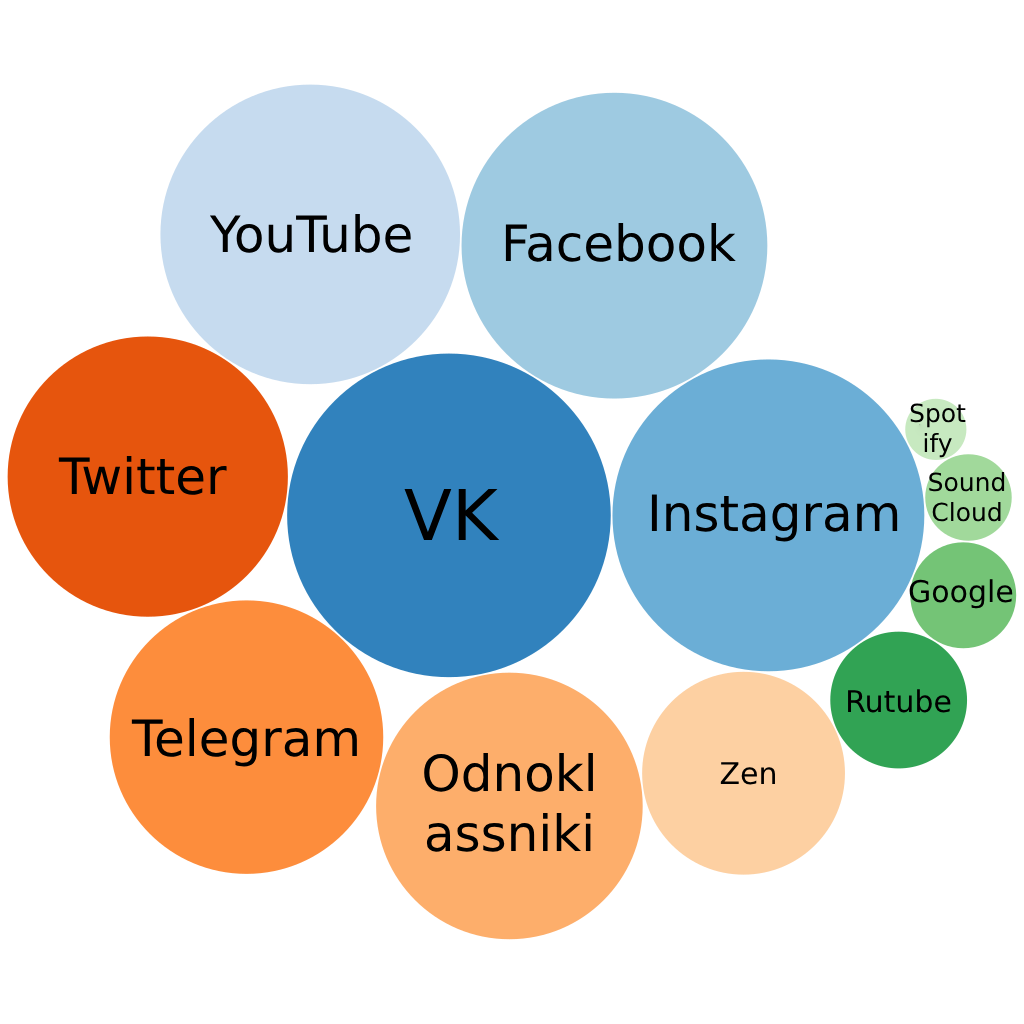
\includegraphics[width=1\linewidth]{chapter/radio_station/Number_of_social_media_accounts_2.png}}
\vspace{-7pt}
\caption{Пузырьковая диаграмма популярности социальных сетей по числу в них аккаунтов радиостанций, СМИ и вещательных каналов на 2024 год}%
\label{fig:radio_station_acc}
\end{marginfigure}

%
